\documentclass[letterpaper,12pt,fleqn]{article}
\usepackage{matharticle}
\usepackage{tikz}
\pagestyle{empty}
\newcommand{\e}{\epsilon}
\begin{document}
\section*{Math-42 Practice Final}

\begin{enumerate}[left=0in]
\item Let \(A=\set{2,3,4}\) and \(B=\set{15,20}\) and defined the relations \(U\) and \(V\) between \(A\) and
  \(B\) as:
  \begin{gather*}
    (x,y)\in U\iff x|y
    V=\set{(2,15),(3,15),(2,20)}
  \end{gather*}
  \begin{enumerate}
  \item Draw a bubble diagram for \(U\).
  \item Is \(U\) a function?
  \item Draw a bubble diagram for \(V\).
  \item Is \(V\) a function?
  \end{enumerate}

\item Consider the following statements:

  \(p\coloneqq\) Max is a cat.

  \(q\coloneqq\) Max is black.

  \(r\coloneqq\) Max is asleep.

  Construct logic expressions for the following compound statements:
  \begin{enumerate}
  \item Max is a black cat but he is not asleep.
  \item Max is neither a cat, black, nor asleep.
  \item Max is a cat but he is not both black and asleep.
  \end{enumerate}

\item Construct a truth table for the logic expression: \(\lnot p\lor q\land r\).

\item Find a counterexample to show that the following statement is false.
  \[\forall\,n\in\N,n^2<2^n\]

\item Let \(C\) be the set of all cats in a shelter and define the following predicates:

  \(B(c)\coloneqq c\) has black coloring.

  \(W(c)\coloneqq c\) has white coloring.

  \(T(c)\coloneqq c\) has tan coloring.

  Express each of the following statements using quantifiers:
  \begin{enumerate}
  \item There is a white cat who is also tan.
  \item Every black cat is also white.
  \item No cats have all three colors.
  \end{enumerate}

\item Which of the following is a negation of: ``all pigs are smart.''
  \begin{enumerate}
  \item Some pigs are smart.
  \item No pigs are smart.
  \item There is at least one dump pig.
  \item All pigs are dumb.
  \item There is at least one smart pig.
  \item Some pigs are dumb.
  \end{enumerate}

\item Let \(A=\set{0,2,4,5,6}\).
  \begin{enumerate}
  \item Negate the statement: \(\forall\,a\in A,\exists,b\in A,a|b\).
  \item Is the original statement true or false?
  \item Is the negation true or false?
  \end{enumerate}

\item Prove: The sum of any two odd integers is even.

\item Show that the following sum is rational by writing it as the ratio two integers: \(\frac{3}{4}+\frac{2}{5}\).

\item Are the following true or false?
  \begin{enumerate}
  \item \(10|0\)
  \item \(0|10\)
  \item \(10|10\)
  \item \(0|0\)
  \end{enumerate}

\item Find the division algorithm of the following integers using 9 as the divisor:
  \begin{enumerate}
  \item \(256\)
  \item \(-256\)
  \end{enumerate}

\item Prove: \(5n+9\) is not divisible by 5.

\item Find a closed form for the sequence:
  \[\frac{1}{2}-\frac{1}{3},\frac{1}{4}-\frac{1}{5},\frac{1}{6}-\frac{1}{7},\frac{1}{8}-\frac{1}{9}\ldots\]

\item Find the first four terms of the sequence \(a_n=3a_{n-1}+1\) with the initial condition \(a_0=5\).

\item Define the family of intervals \(\set{A_i=[0,i):i\in N}\) and evaluate the following:
  \begin{enumerate}
  \item \(\displaystyle\bigcup_{i=1}^4A_i\)
  \item \(\displaystyle\bigcap_{i=1}^4A_i\)
  \item \(\displaystyle\bigcup_{i=1}^nA_i\)
  \item \(\displaystyle\bigcap_{i=1}^nA_i\)
  \item \(\displaystyle\bigcup_{i=1}^{\infty}A_i\)
  \item \(\displaystyle\bigcap_{i=1}^{\infty}A_i\)
  \item Are the \(A_i\) mutually disjoint, and if so then why specifically?
  \end{enumerate}

\item Draw the Venn diagram showing the included regions in \(A\cap(B\cup C)\).

\item Consider a function \(f:A\to B\) represented by the following diagram:

  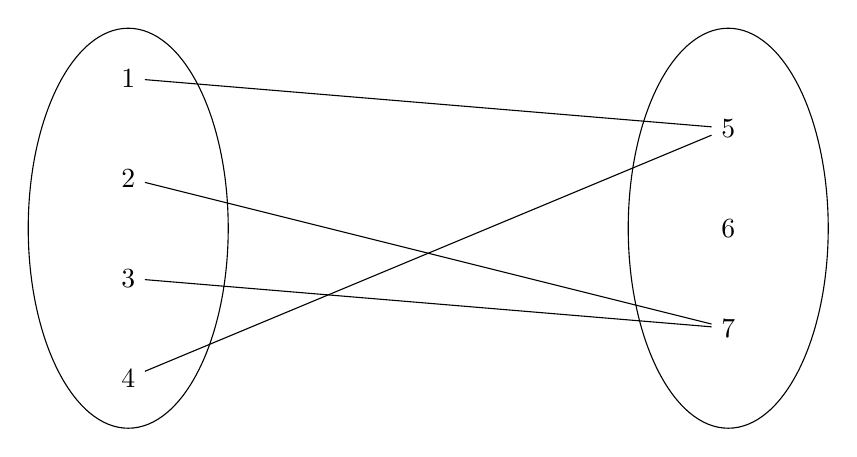
\begin{tikzpicture}
    \draw (0,0) ellipse(0.5in and 1in);
    \draw (3in,0) ellipse(0.5in and 1in);
    \node (a1) at (0,0.75in) {\(1\)};
    \node (a2) at (0,0.25in) {\(2\)};
    \node (a3) at (0,-0.25in) {\(3\)};
    \node (a4) at (0,-0.75in) {\(4\)};
    \node (b5) at (3in,0.5in) {\(5\)};
    \node (b6) at (3in,0) {\(6\)};
    \node (b7) at (3in,-0.5in) {\(7\)};
    \draw (a1) -- (b5);
    \draw (a2) -- (b7);
    \draw (a3) -- (b7);
    \draw (a4) -- (b5);
  \end{tikzpicture}

  \begin{enumerate}
  \item Write \(f\) as a set of ordered pairs.
  \item What is the domain of \(f\)?
  \item What is the codomain of \(f\)?
  \item What is \(f(3)\)?
  \item What is the range of \(f\)?
  \item What is the image of \(\set{1,4}\)?
  \item What is the preimage of \(\set{5,6}\)?
  \end{enumerate}

\item US phone numbers are of the form NDD--NDD--DDDD where \(N\) is a digit from \(2\) to \(9\) and
  \(D\) is a digit from 0--9.
  \begin{enumerate}
  \item How many possible phone numbers are there?
  \item How many possible phone numbers are there that start with \(800\)?
  \item How many possible phone numbers are there if the digits within each part are distinct?
  \end{enumerate}

\item Suppose that you have 10 pairs of socks of different colors all jumbled up in your drawer.  What is the
  minimum number of socks that you need to select from the drawer to ensure that you have a pair of the same
  color?

\item A committee of 4 people must be selected from a staff of 10 people: 6 men and 4 women.
  \begin{enumerate}
  \item How many ways are there to select a committee?
  \item How many ways to select a committee of 2 men and 2 women?
  \item How many ways to select a committee with at least 1 woman?
  \item How many ways to select a committee with at most 2 men?
  \item How many ways are there to select a committee if Bill and Ted refuse to work together?
  \item How many ways are there to select a committee if Bill and Joy must either both serve or not serve?
  \end{enumerate}

\item You take 10 cards out of a standard deck: 6 red (D,H) and 4 black (C,S).  You shuffle the 10 cards well and
  then select 2 at random.
  \begin{enumerate}
  \item Construct a decision tree for the probabilities associated with this experiment.
  \item What is the probability that both cards are red?
  \item What is the probability that both cards are black?
  \item What is the probability that a black followed by a red is selected?
  \item What is the probability that second card is black?
  \end{enumerate}

\item What is the minimum number of integers that must be selected between 0 and 10 to ensure that at least one
  is odd?

\item Consider the numbers from 1 to 100.
  \begin{enumerate}
  \item How many are multiples of 5 or 6?
  \item If a number is selected randomly, what is the probability that it is a multiple of 5 or 6?
  \item If a number is selected randomly, what is the probability that it is not a multiple of 5 or 6?
  \end{enumerate}

\item Consider the word ``ONWARD'':
  \begin{enumerate}
  \item How many ways are there to arrange the letters?
  \item How many ways are there to arrange the letters if WR must remain together in that order?
  \item How many ways are there to arrange the letters if WR must remain together in either order?
  \end{enumerate}

\item Suppose you flip a fair coin 4 times.
  \begin{enumerate}
  \item Describe the sample space using setbuilder notation.
  \item Describe the sample space using roster notation.
  \item What is the probability of exactly one heads?
  \item What is the probability of at least two heads?
  \end{enumerate}

\item Let \(f,g:\Z\to\Z\) be defined by \(f(n)=n\bmod2\) and \(g(n)=n+3\).  Evaluate:
  \begin{enumerate}
  \item \((f\circ g)(5)\)
  \item \((g\circ f)(5)\)
  \item \((f\circ f)(5)\)
  \item \((g\circ g)(5)\)
  \end{enumerate}

\item Consider the function of problem 17.
  \begin{enumerate}
  \item Is \(f\) injective (one-to-one)?
  \item Is \(f\) surjective (onto)?
  \end{enumerate}

\item Prove: \(f(x)=e^{2x+1}\) is injective (one-to-one).

\item Negative the following statement:
  \[\forall\,\e>0,\exists\,N\in\N,\forall\,n\in\N,(n>N\implies\abs{x_n-x}<\e)\]

\item The following is a rigorous proof of \((p\lor\bar{q})\land(p\lor q)\equiv p\).  Justify each of the steps.
  \begin{align*}
    (p\lor\bar{q})\land(p\lor q) &\equiv p\lor(\bar{q}\land q) \\
    &\equiv p\lor F \\
    &\equiv p
  \end{align*}
\end{enumerate}

\end{document}
